\begin{frame}{revisiting congestion collapse}
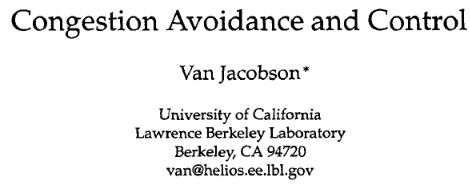
\includegraphics[width=0.6\textwidth]{../congest/jacobson-title}
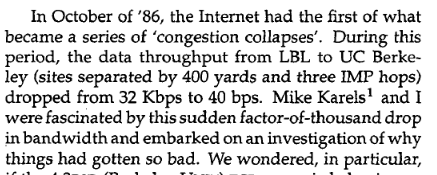
\includegraphics[width=0.6\textwidth]{../congest/jacobson-disaster}
\end{frame}

\begin{frame}<1>[label=jacobsonFixes]{fixes from Jacobson's 1987 paper}
\begin{tikzpicture}
\node[anchor=north west] (fixes) at (0, 0) {
    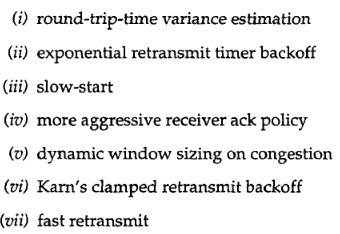
\includegraphics[width=0.6\textwidth]{../congest/jacobson-fixes}
};
\path[draw,help lines] (0, 0) grid[step=1] (8, -5);
\begin{visibleenv}<2>
    \draw[red,ultra thick] (0, -3.8) rectangle (9, -4.4);
\end{visibleenv}
\begin{visibleenv}<3>
    \draw[red,ultra thick] (0, -2) rectangle (5, -2.8);
\end{visibleenv}
\end{tikzpicture}
\end{frame}
